
\documentclass[12pt]{article}
\usepackage[a4paper, margin=.30in]{geometry}
\usepackage{graphicx ,
            wrapfig,
            xcolor, 
            enumerate,
            amsmath,
			fontenc,
			tcolorbox,circuitikz,tikz,bm
            }
			\usepackage{pgfplots}
\pgfplotsset{compat=newest}
\usepgfplotslibrary{fillbetween}
\usepackage{pgfplots}
\newcommand\headerMe[2]{\noindent{}#1\hfill#2}
\renewcommand{\thesection}{\Roman{section}}

\author{Zakaria HAOUZAN}
\date{\today}

\begin{document}
% headers --------------
\headerMe{Matière : Physique-Chimie}{Professeur : Zakaria HAOUZAN}\\
\headerMe{Unité : Mécanique }{Établissement : Lycée SKHOR qualifiant}\\
\headerMe{Niveau : 2BAC-SM-PC}{Heure : 5H}\\

% ------Content ________
\begin{center}

    \Large{Leçon $N^{\circ} 17 $: \color{red}Atome et mécanique de Newton}
\end{center}

%\begin{center}

	%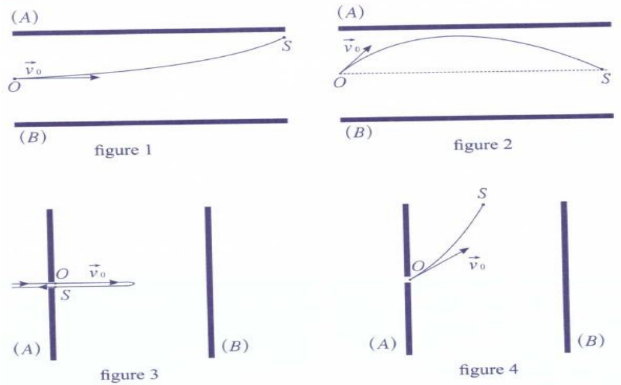
\includegraphics[width=0.6\textwidth]{./img_02.png}
%\end{center}



%\begin{wrapfigure}{r}{0.3\textwidth}
	%\vspace{-2cm}
	%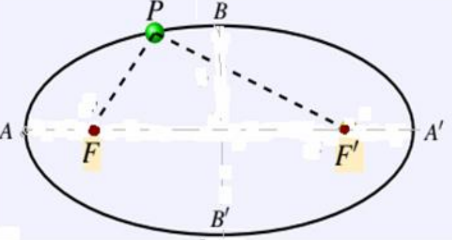
\includegraphics[width=0.3\textwidth]{./img_00.png}
%\end{wrapfigure}

\section{Limites de la mécanique de Newton:}
\subsection{Loi de Newton et loi de Coulomb:}
\subsubsection{Interactions gravitationnelles : loi de Newton:}
Deux corps A et B de masses mA et mB exercent l'un sur l'autre des forces d'attraction gravitationnelle de même intensité :
\begin{center}

	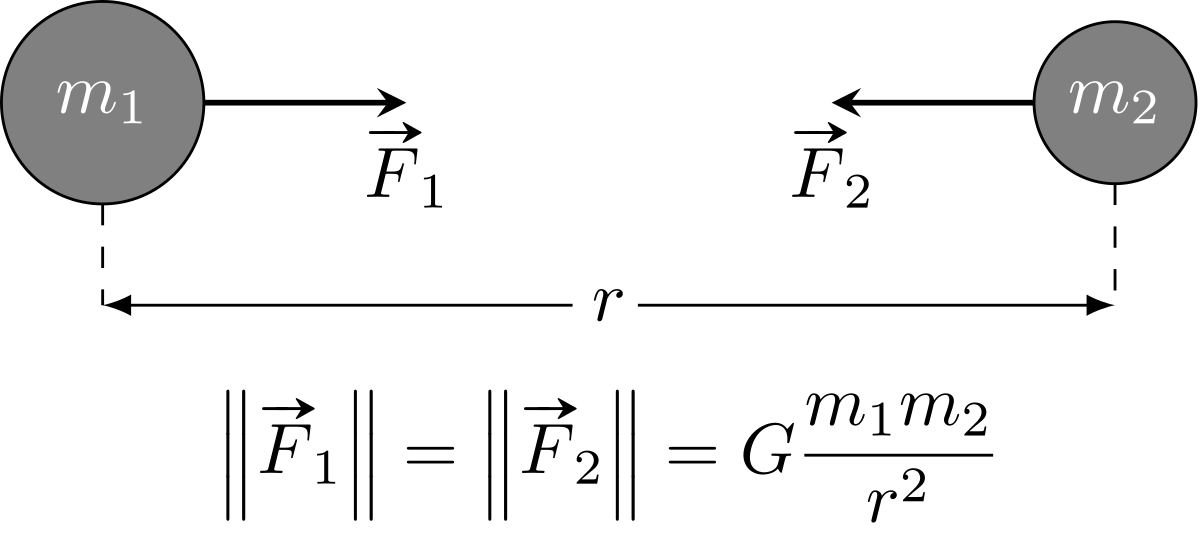
\includegraphics[width=0.3\textwidth]{./grav.png}
\end{center}


\subsubsection{Interactions électrostatiques : loi de Coulomb:}
La force d'attraction électrostatique entre l'électron de charge qE et le noyau de charge qN et est donnée par la relation suivante:
\begin{center}

	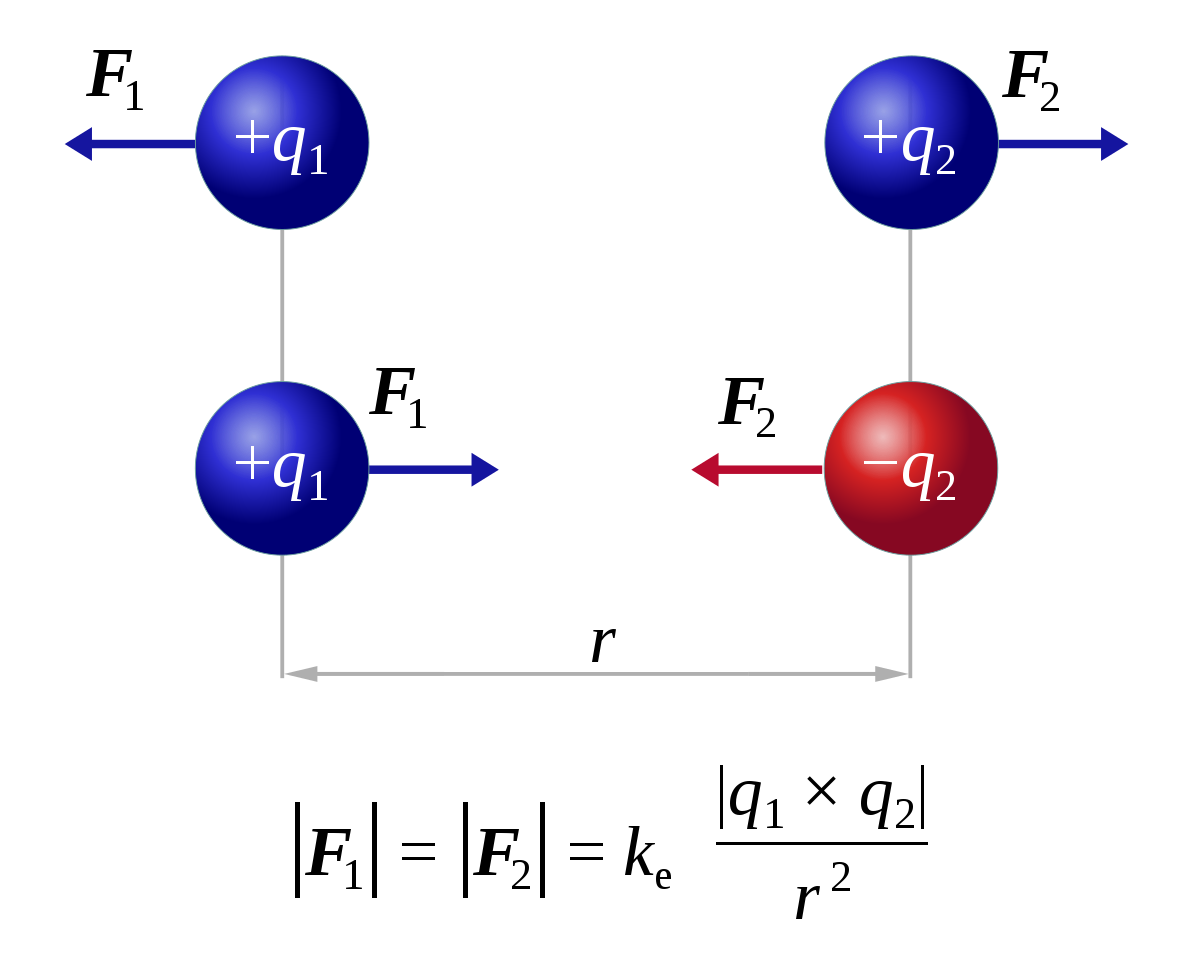
\includegraphics[width=0.3\textwidth]{./electroStatique.png}
\end{center}
\subsection{Limites de la mécanique de Newton:}
En se basant sur les lois qui gèrent les forces d'attractions électrostatiques et celle qui gèrent les forces d'attractions
gravitationnelles Rutherford a proposé en 1907 le modèle planétaire de l'atome (Un noyau positivement chargé autour duquel
gravitent des électrons).



Mais la force principale intervenant dans les atomes n'est pas celle de la gravitation (car les planètes tournant toutes dans le
même plan et dans le même sens n'est pas possible avec des électrons qui se repoussent) .En plus dans ce modèle en tournant les
électrons perdraient peu à peu leur énergie pour finir par tomber sur le noyau. Le modèle basé sur la mécanique de Newton est en
plus incapable de rendre compte de certains phénomènes, comme les spectres de raies . Par conséquence il y'a apparition de la
mécanique quantique.

\section{Quantification des échanges d'énergie:}
\subsection{Notion de quantification de l'énergie:}
Lorsque la matière absorbe ou émet de l'énergie par rayonnement, elle ne peut échanger que des paquets d'énergies multiples
entiers de $h.\nu$ d’où quantification de l'énergie.
La charge qE de l'électron et la charge qN du noyau sont de signent contraires.

\subsection{Quantification de l'énergie dans les atomes:}
Lorsqu'un atome est à son niveau d'énergie le plus bas, il est à son état fondamental : c'est l'état le plus stable.
L'atome peut passer d'un état à un autre état en gagnant ou en perdant de l'énergie.

Pour expliquer cet échange d'énergie entre l'atome et le milieu extérieure, Bohr a supposé que l'énergie de l'atome est quantifiée et
il a proposé la relation $E_n = \frac{-E_0 }{n^2}$ qui permet de déterminer les différents niveaux de l'atome d'hydrogène

(Dans cette relation le nombre quantique principal "n" est un nombre entier non nul et $E_0=13,6eV$ )

\underline{Le premier niveau d'énergie qui correspond à n=1}: est l'état fondamental il correspond au plus bas niveau d'énergie de l'atome d'hydrogène son énergie $E_1 = \frac{-E_0}{1^2} = -13,6ev$

Les niveaux d'énergie $n > 1$ Correspondent à des niveaux excités :

\begin{itemize}
	\item Pour n=2 l'atome est excité au 2 niveau d'énergie $E_2 = -\frac{13,6}{2^2}$
	\item Pour n=3 l'atome est excité au 3 niveau d'énergie $E_3 = -\frac{13,6}{3^2}$
	\item Pour n=4 l'atome est excité au 4 niveau d'énergie $E_4 = -\frac{13,6}{4^2}$
	\item Pour n=5 l'atome est excité au 5 niveau d'énergie $E_5 = -\frac{13,6}{5^2}$
	\item Pour n=6 l'atome est excité au 6 niveau d'énergie $E_6 = -\frac{13,6}{6^2}$
	\item Pour n=$\infty$ l'atome est excité au $\infty$ niveau d'énergie $E_{\infty} = 0$
\end{itemize}

\begin{center}

	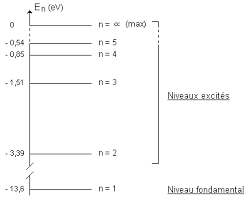
\includegraphics[width=0.4\textwidth]{./diagramme.png}
\end{center}

\subsection{Le photon: }
Pour explique le phénomène de l'effet photoélectrique (Extraction des électrons d'un métal par un rayonnement)Albert Einstein a considéré en 1905 que la lumière possède une nature corpusculaire c'est-à-dire qu'un faisceau lumineux de fréquence $\nu$ est
constitué de photons, grains élémentaires et que chaque photon a pour énergie 

$$E=h.\nu$$

\begin{itemize}

	\item h: Constante de Plank $h=6,63.10^{-34}$
	\item $\nu $ : la fréquence de la lumière $\nu = \frac{c}{\lambda}$
	\item c : la célérité de la lumière  dans le vide
\end{itemize}

\subsection{Postulats de Bohr: }
Le modèle de Bohr de l'atome:
\begin{itemize}
	\item L'électron tourne autour du noyau de l'atome dans des niveaux d'énergies quantifiés.
	\item L'atome n'existe que dans des niveaux d'énergies bien déterminés.
	\item Les variations d'énergie d'un atome sont quantifiées.
\item Lorsque l'électron passe d'un niveau Ep à un niveau d'énergie inférieure En , il émis un rayonnement de fréquence $\nu$ telle que: $E_p - E_n = h.\nu$




\end{itemize}
\begin{center}

	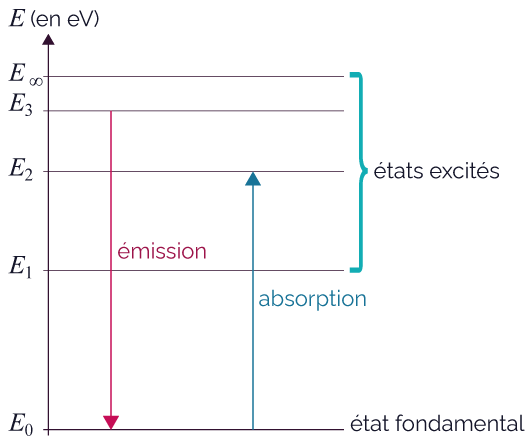
\includegraphics[width=0.4\textwidth]{./absorEmission.png}
\end{center}
\section{Spectre d'émission et spectre d'absorption:}


\subsection{Spectre d'émission de l'atome d'hydrogène:}

\subsubsection{  Expérience de Balmer}

Par décharge électrique dans une ampoule contenant le gaz dihydrogène on obtient le spectre d'émission de l'atome d'hydrogène:
c'est un spectre de raies discontinu, il contient quatre raies visibles:

L'examen du spectre d'émission montre qu'il contient d'autres raies invisibles.

\begin{center}

	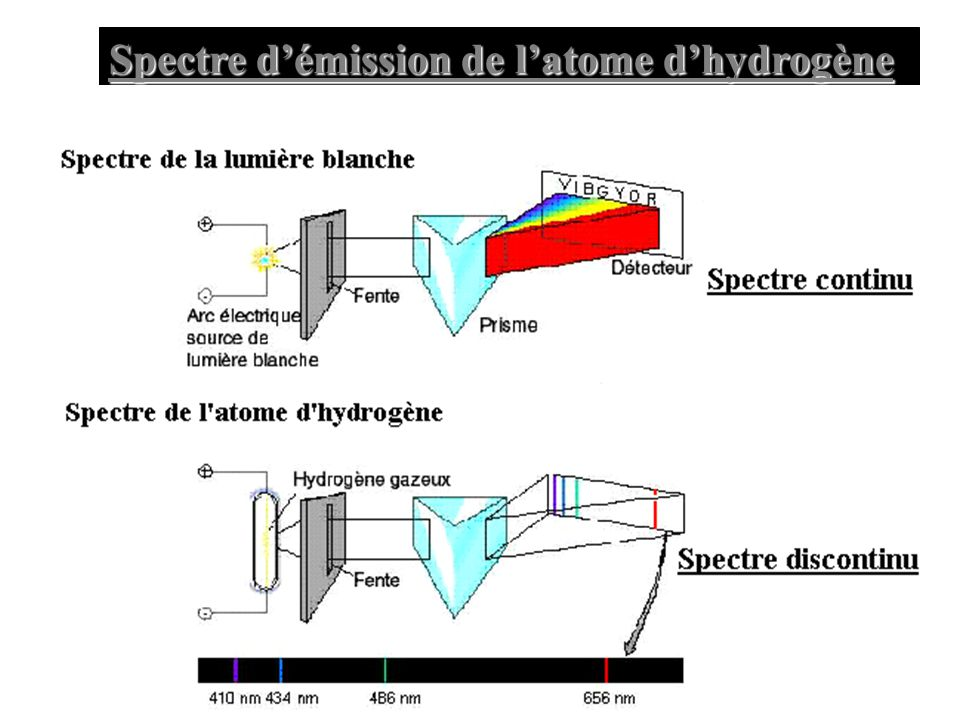
\includegraphics[width=0.4\textwidth]{./Blamer EXp.jpg}
\end{center}


\subsubsection{Interprétation:}
Par excitation avec la décharge électrique l'électron de chaque atome d'hydrogène passe à un niveau d'énergie plus élevé (les
atomes sont dits excités) par la suite ces électrons perdent leurs excitations en passant à un niveau d'énergie plus bas. Cette
transition entraine l'émission de radiations de longueurs d'ondes bien déterminées et on obtient le spectre d'émission.
La relation qui correspond au passage de l'atome excité d'un niveau d'énergie Ep à un niveau d'énergie inférieure En est:

On obtient la longueur d'onde de la radiation émise :
$$\frac{1}{\lambda} = \frac{E_0}{h.\nu}(\frac{1}{n^2} - \frac{1}{p^2})$$

On pose $R_H = \frac{E_0}{h.\nu} \approx 1,0097.10^7$

\section{Les séries de spectre d'émission de l'atome d'hydrogène:}
\subsection{Série de Balmer}

Après plusieurs recherches Balmer a déterminé les longueurs d'ondes des radiations émises par l'atome d'hydrogène excité
tout en considérant que les électrons en perdant leurs excitations passent d'un niveau d'énergie  p  au 2ème niveau d'énergie :n=2
avec p>2.
\begin{center}

	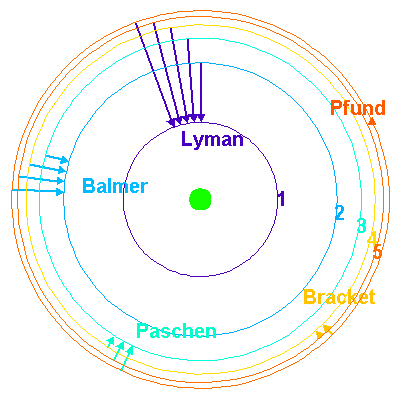
\includegraphics[width=0.4\textwidth]{./series.png}
	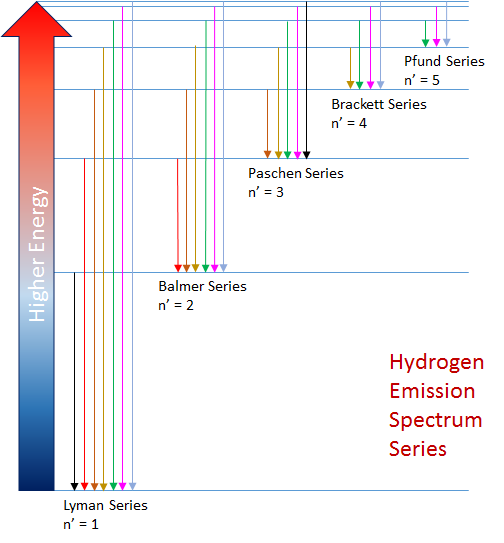
\includegraphics[width=0.4\textwidth]{./series2.png}

\end{center}
\end{document}

